\documentclass[11pt]{article}
% \usepackage[usenames,dvipsnames,svgnames]{xcolor}

\usepackage{deauthor}
\usepackage{times, enumerate}
\usepackage{graphicx}
\usepackage{authblk}
\usepackage{hyperref,subfigure}
\usepackage{wrapfig}
\usepackage{enumitem}



\begin{document}

\title{Slowing the Spread of Infectious Diseases Using Crowdsourced Data}
%
\author{Sydney Von Arx, Isaiah Becker-Mayer, Daniel Blank, Jesse Colligan, Rhys Fenwick, Mike Hittle, Mark Ingle, Oliver Nash, Victoria Nguyen, James Petrie, Jeff Schwaber, Zsombor Szabo, Akhil Veeraghanta, Mikhail Voloshin, Tina White, Helen Xue} 
% \affil{{\small \texttt{\{sseb,biessman,tjnsch,dsalina,seufert,szarvasg
% \}@amazon.com}}}
% \affil{Amazon Research}

\maketitle

% \begin{abstract}
% Contact tracing is a critical part of reopening society. While manual contact tracing by medical professionals is essential, there’s growing acknowledgement that supplementing this with digital approaches might make a significant difference in the speed with which we can reopen.
 
% Safe Paths is open source, standards-based, privacy-first framework that works closely with public health entities. Our approach is to roll out apps, SDKs, privacy-preserving network backbones, and interoperable protocols, so that any developer can build experiences that perform contact-tracing and related activities in safe, easy to use ways.

% In this paper, we’ll compare some of the existing technologies that can be used to aid contact tracing and exposure notification efforts, and make the case for using a holistic, multi-modal approach rather than relying exclusively on a single technology.
% \end{abstract}

\section{Introduction}

We are a group of volunteers --- researchers, software engineers, privacy and public health experts --- who have developed a privacy-preserving mobile app intervention to reduce the spread of COVID-19. Our mobile app performs automatic decentralized contact tracing using bluetooth proximity networks. 

Our volunteers care strongly about preserving human life and human rights. All data we could collect is voluntary and fully anonymized. All code is transparent. It is open source~\cite{covidwatch} and could be easily reviewed, reproduced and used anywhere on the planet.

The app could be installed by anyone with a bluetooth-capable smartphone, alerting them to their risk of having been in contact with a confirmed case of COVID-19, and helping them to protect themselves and their friends, families, and other contacts altruistically.

We believe scalable measures like an app are especially helpful in communities where contact tracing resources are too limited to match the scope of the pandemic. We're building this app to provide components and tools that public health agencies can use to supplement their pre-existing efforts to fight COVID-19, assisted by voluntary public action. 


\subsection{Privacy Focus}

Existing mobile apps without a privacy focus have been an effective intervention to reduce the spread of COVID-19. However, invasive interventions carry significant human rights costs, including the temporary loss of personal freedom and fears around whether that freedom will be restored.

A mobile app with a strong privacy model may also have greater efficacy because people will be more likely to share accurate data if they know that data is safe. Ensuring privacy prevents COVID-19 patients from being ostracized or socially harmed on account of inadvertent potential data exposures. Also, mobile apps with poor privacy models may further undermine public confidence in responses and exacerbate existing mistrust. 

In contrast, our mobile app research has focused on developing a strong privacy model while still providing effective intervention. Using the app, users can alert recent contacts without anyone being able to trace the information back to them. We believe this intervention has the potential to slow or stop the spread of COVID-19 and save lives. 

\subsection{Current Mobile Phone Interventions}


South Korea and China have demonstrated two successful systems for containing COVID-19 that make extensive use of technology. The results they have seen match well with predictions from numerical models: with a sufficient diagnosis rate and contact tracing accuracy COVID-19 can be contained.

China~\cite{mcneil_2020} was the first to create a mobile app intervention. Their app uses GPS history and other data to assign a risk score. This score is then used to control which individuals are allowed to move freely. China’s intervention appears to have been successful, but required far-reaching state surveillance that, by the standards of most liberal democracies, would be considered highly invasive, likely unlawful, and politically unpalatable.


South Korea~\cite{normile_2020} publicizes a large amount of information collected from the cellphones of infected patients so that others can determine if they had been in contact. South Korea’s success has been attributed mostly to (1) widespread testing (2) contact tracing and (3) case isolation. However, their mobile alert solutions do not effectively anonymize patient data. They gather location data from interviews, mobile phone GPS history, surveillance cameras, and credit card records then send text alerts with the location history of patients. Much like the intervention in China, this appears to be effective, but takes a similarly high toll on personal privacy.


We’ve built a privacy-preserving version of these successful interventions that we believe would have a regulatorily, publicly, and politically viable adoption process within the United States and other Western countries. The system as designed complies with existing regulations around medical information in the United States and does not reveal identifying patient information. 


\subsection{Making Interventions More Efficient}

Non-pharmaceutical pandemic interventions fundamentally make a trade-off between two important social goods: (1) loss of life from the pandemic and (2) economic impact, which influences health and well-being outcomes indirectly. Mobile app interventions are a powerful public health tool because they can improve this trade-off.


In general, non-pharmaceutical approaches to infectious disease control have the following components:
\begin{itemize}
\item Filtering (picking a subset of the population)
\item Intervention (modifying the behaviour of these people)
\end{itemize}
For example, quarantining patients with a positive diagnosis applies a filter based on testing and then applies the quarantine intervention. Other examples include travel restrictions for at-risk areas, cancelling public events in a specific city, or encouraging more handwashing in an entire country. Some of these interventions, especially self-isolation, are highly effective~\cite{ferguson} at preventing the transmission of infectious diseases like COVID-19. The downside is that they can also be costly to use.



The quality of filtering plays a crucial role in determining the trade-off between loss of life and economic impact. If filtering is poor, a correspondingly larger economic impact will be needed to achieve the same loss of life reduction. Without good filtering, broad quarantines and social distancing are needed, incurring a huge cost in the form of negative impact on people’s lives.


Unfortunately, traditional approaches to filtering, such as contact tracing, are labor intensive and don’t scale well. So we expect filtering (and, correspondingly, the trade-off between loss of life and economic impact) to degrade in quality as a pandemic grows. But automated contact tracing solutions have the potential to be more scalable -- and potentially even more accurate, with access to higher quality information than traditional contact tracing. This may allow for a better trade-off to be maintained in the midst of a pandemic.




\section{Proposed System: Three Parts}

The system proposed here is intended to be used as part of a broader campaign to combat COVID-19 immediately and in the long term. These methods focus on gathering and disseminating the information needed to perform targeted interventions. 

There are three components to this system that work almost independently, but can be bundled into a single mobile app. Depending on privacy requirements and the needs of specific public health authorities a subset of these capabilities could be utilized.

\begin{enumerate}
  \item Automated contact tracing at scale using anonymized bluetooth proximity sensing 
  \item Heatmap informed by epidemiological models using anonymized GPS data to warn users about high risk areas
  \item Recommendations from local health authorities and risk-aware suggestions about when to get tested
\end{enumerate}

\section{Part 1: Bluetooth Contact Tracing}

\subsection{Contact Tracing Background}

Non-pharmaceutical methods focused on social distancing reduce the spread of COVID-19. These methods are based on reducing contact between infected and susceptible people, even when it isn’t known who is infected. 
In the simplest form, this is being achieved by reducing all social events and increasing precautions like handwashing. This is an effective measure because the number of new infections is roughly proportional to the number of contact events with infectious people.


A more targeted approach employed by many health agencies is contact tracing~\cite{contacttracing_ca}. This system works by finding and monitoring contacts of patients that have been diagnosed. Individuals that are thought to be infected are then put into isolation to prevent further transmission, and individuals who have previously been in contact with infected individuals are quarantined.

\begin{figure}[h]
\centering
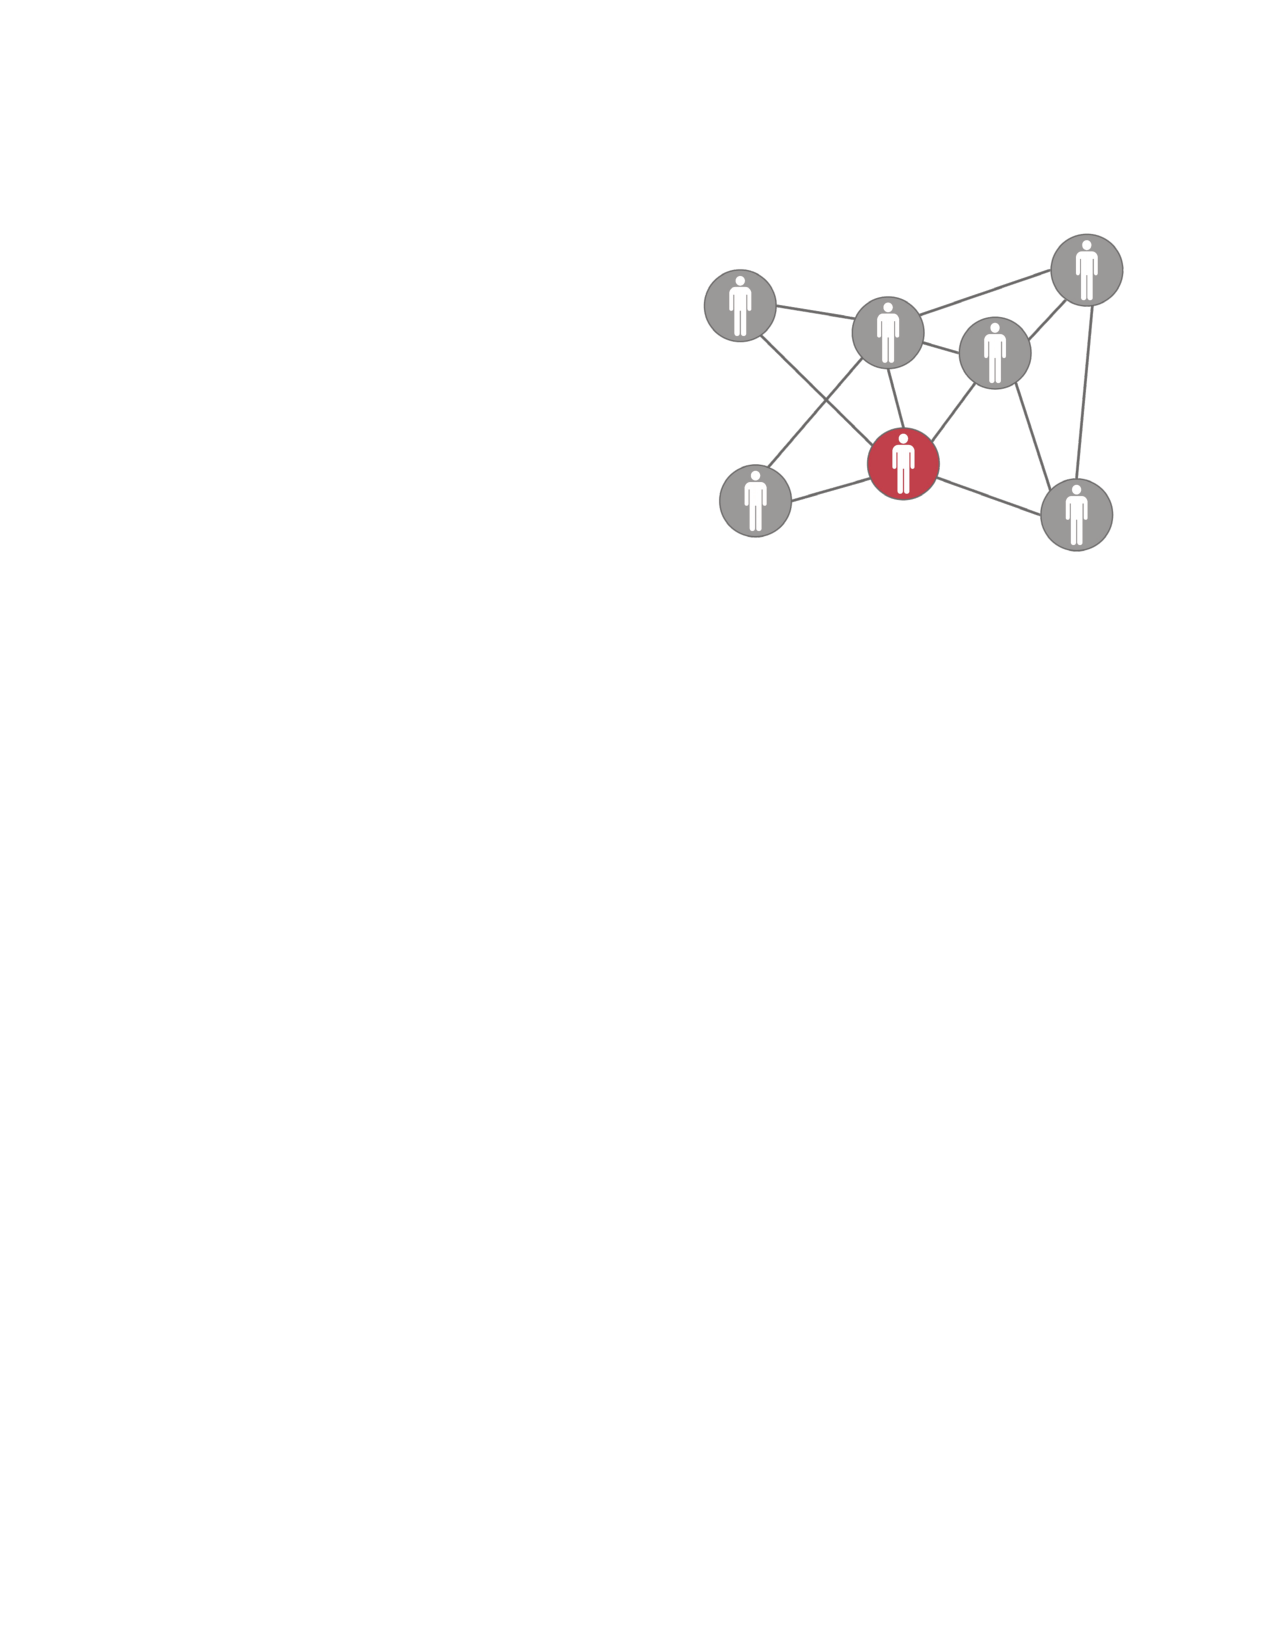
\includegraphics{figs/fig2.pdf}
\caption{Contact Network}
\end{figure}

Hellewell et al.~\cite{lancet} analyzed the effectiveness of contact tracing as a method to contain COVID-19 at the beginning of an outbreak. \textbf{Their findings are promising: with 80\% contact tracing accuracy and a mean detection time of 3.8 days after symptom onset, containment is likely.}

In the context of contact tracing, there are three parameters that models show~\cite{Ferrettieabb6936} can strongly impact results:
\begin{enumerate}
\item Reduction in overall transmission through social distancing
\item Testing rate and time to diagnosis
\item Contact tracing accuracy
\end{enumerate}

\subsection{Model Description}

Mobile phones are carried by a majority of people in several countries with an estimated 3.5 billion users worldwide. They are extremely common in Western society, with over 70\% of the US population estimated to own one. Bluetooth is a radio protocol that can be used to wirelessly communicate between nearby mobile devices and the signal strength can be used to estimate distance.


Mobile devices can be made to proactively record contact events with other nearby devices by sending bluetooth signals. By measuring the signal strength and discrete number of contact events, the duration and distance of contact between two phone users can be estimated. 



By recording all contact events, a high accuracy list of at-risk individuals can be generated automatically when a new person is diagnosed. These individuals can then be immediately notified to ensure they self-isolate before infecting more people. 

\textbf{Bluetooth proximity may be the most accurate crowdsourcing method for approximating close contact to perform contact tracing.}


While GPS data is a more well-known general technology, there are significant advantages bluetooth has over GPS in terms of accuracy for contact tracing. With bluetooth, proximity can be approximated by signal strength that is reduced by obstructions like walls; therefore, it more accurately reflects functional proximity in high-risk environments for close contact: inside buildings, in vehicles and airplanes, and in underground transit.


\textbf{Bluetooth communication also occurs directly between mobile devices. This means a decentralized system can be built more easily with and with stronger privacy protection than other crowdsourcing data types like GPS trajectories. }


We are also pursuing research in developing inexpensive external bluetooth devices under the same automatic contact tracing alert system for use in communities with fewer smartphone users. These methods would face much steeper adoption challenges, but if mobile app users and external device users could be integrated under a single system, outcomes could be further improved over more global communities. 

\subsection{Privacy Model}

The bluetooth contact tracing system (Fig~\ref{privacymodel}) can be structured in a decentralized and anonymous way using randomly generated and locally stored ‘Contact Event Numbers’. This allows the system to function fully without any private information being stored or transmitted. 

By generating a new random number for each contact event, the system is able to operate without storing or transmitting any personal information. This method is designed so that only the phones involved in a contact event are able to identify messages on a public database.


\begin{figure}[ht]
\centering
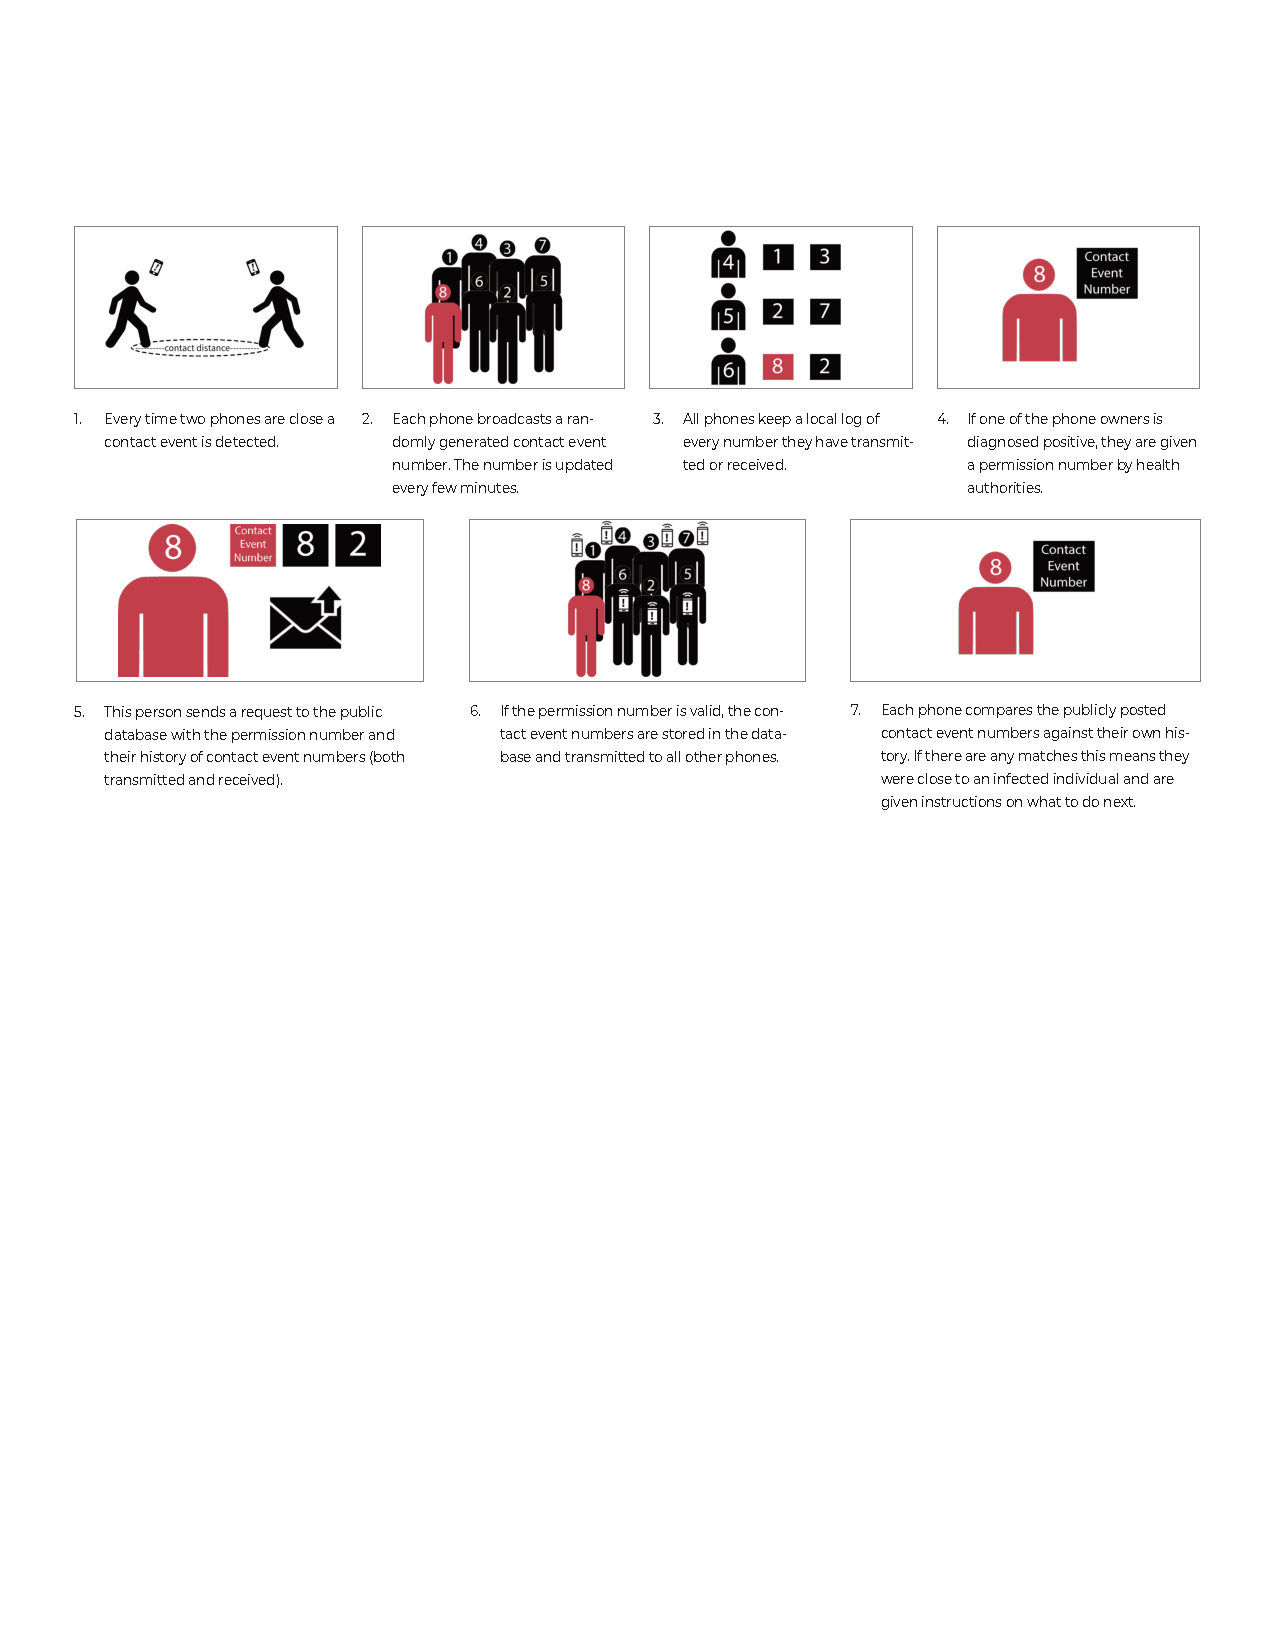
\includegraphics[width=\textwidth]{figs/fig3.pdf}
\caption{Privacy Model}
\label{privacymodel}
\end{figure}




The only authentication required is the permission number provided by a public health authority. This permission number is used so that malicious actors cannot send false alarms. After authentication, the permission number is deleted from server memory.

The contact event numbers are random and only known by the message recipients and the message sender, so the database can be made public without risk of sensitive information being discovered. 
While our current intervention is based on permission numbers, in regions where widespread testing is unavailable, a well-designed symptom sharing questionnaire may perform a similar function, with a higher number of false positives. Research in this direction is currently being done by the CoEpi team. 
The most effective form of this intervention would occur in communities that implement widespread testing and where permission numbers are shared with the mobile app by public health departments. 


\subsection{Database}


The specification for the database is very simple: it is shared across all installations of the app and stores anonymized Contact Event Numbers. If protections against hoaxes are required, permission numbers can be used, but they are not required for the privacy model. If the database grows too large, it can also be fragmented based on general location. The code and a more in depth discussion of architecture are available on the open source github repo~\cite{covidwatch}.

\subsection{Implementation}

Bluetooth contact tracing is implemented via background processes on iOS and Android. The approach currently being investigated utilizes BLE functionality for background advertisement and scanning. Due to different system requirements for Android and iOS, the protocol works differently depending on the operating systems of the devices involved. The key challenges are:

\begin{enumerate}
\item iOS devices acting as ``peripherals'' in the background can only be found by ``centrals'' that are scanning for their specific service UUID. These peripherals must establish a connection to transfer any data.
\item Android devices have several unfixed bugs where subsequent connections with many devices can cause the bluetooth system to lock up.
\end{enumerate} 


The current solution is a hybrid model that is asymmetric for communication between iOS and Android. All devices will simultaneously act as peripherals and centrals, but only some devices will be able to detect others, and only some devices will need to establish a connection to exchange data. An extended description of the communication model and the code are available on our Github repo~\cite{covidwatch}. This model has been successfully implemented as a proof-of-concept.

\section{Part 2: GPS Heatmap}

\subsection{Model Description}

GPS capability is ubiquitous among smartphone devices, and high-resolution spatiotemporal data is regularly used by mapping and social media apps. Given anonymised GPS data along with user infection status, we can approximately calculate where the fomite-based risk of infection is the highest; meaning, where there may be inanimate objects capable of transmitting infection. 
Anonymized GPS data can inform an epidemiological model to show how the disease is likely to spread.
Based on this epidemiological model, we can generate a risk heatmap showing comparative fomite risk for different geographical areas at the current time. This heatmap enables our users to adjust their behaviours in response to their local environment. They could, for example, choose to take extra precautions when in high-risk areas, or avoid them altogether. This both decreases the risk of our users becoming infected, and decreases the risk that they will infect those around them.
This provides a supplementary service for our users to inform their social distancing measures.


\subsection{Epidemiology Model}

To describe it simply, the heat map builds upon SEIRS models~\cite{seirs}. 
% and simulates users according to the following state machine:
The population of simulated users, and probability and timing of a simulated user moving from one state to the next, are generated from the data we have available: both on the background demographics of impacted areas and specific case data. 
Each simulated user is given an age and has a chance of having pre-existing health conditions, which impact their contagiousness and susceptibility to infection.
The anonymised user trajectories are superimposed over a grid covering the area being modeled, while the grid squares are filled with a number of randomly generated simulated humans based on demographic data for that area. As simulated infected and contagious users move across the grid, they carry a chance of infecting the other simulated humans (both user and non-user) sharing their grid space at any given time. 
Simulated non-user humans also have a probability of adjusting their behaviour and movement throughout the simulation, to model hospital admission and self-isolation.
This simulation is run multiple times, and the amount of time each infected human spent in each grid square contributes to its overall risk score, which is represented by the final heatmap.
As our understanding of COVID-19 progresses, this heatmap can be refined, and the parameters tuned to more accurately reflect real-world data.


\subsection{Privacy Model}


Given the personally identifying nature of the spatiotemporal trajectories provided by GPS systems, this information will be handled in a more complex way involving two distinct servers.
The first server, Server A, will handle anonymisation using the methods described in the following GPS Anonymization Model section. Users will send their GPS data to Server A first without any other information, and Server A will return the now-anonymised data to them.
They will then upload the anonymised data, along with their infection status, to the second server, Server B. Server B will take this data and add it to our epidemiological simulation, generating a heatmap.


\subsection{GPS Anonymization Model}

The heatmap may either require the application of an anonymization algorithm, or the explicit consent of users to publish high resolution GPS trajectories. There is a large body of academic work~\cite{Primault_2019} behind the anonymisation of spatiotemporal data, most of which draw from a handful of common strategies. These include aggregating multiple similar trajectories together, decreasing the resolution of each datapoint across space and time, removing particularly distinctive datapoints, and swapping sections of trajectories that cross paths.


Of the several metrics used for quantifying de-identification methods, we have chosen k-anonymization. A dataset is anonymous for some integer k if no entry can be narrowed down further than belonging to one of k individuals. For example, a group of trajectories would be 3-anonymous if each trajectory could plausibly belong to at least 3 individuals. Our aim is to create a dataset with the maximum possible k-value that still preserves utility. The worst-case scenario we would be willing to publish is at minimum a 10-anonymous dataset with respect to an adversary using commonly available geographical information. 


Given the urgency of the situation, we intend to use contractual boundaries against deanonymization rather than aiming to protect against more sophisticated and hypothetical attacks on our anonymization scheme. Building anonymity systems that are resistant to more sophisticated attacks is challenging, and takes much more time.



The anonymisation model we are implementing is one created by \cite{traject}. It allows for flexible k-anonymity without significant distortion, and has a proven and open-source implementation.
This does require a significant number of trajectories to be accurate, so we will be supplementing our initial database with plausible synthetic trajectories created by the Brinkhoff trajectory generator.
The end result is that the trajectories being used to generate our heatmap can be mathematically verified to be anonymous, guaranteeing the privacy of our users.


\section{Part Three: User Recommendations}



We have designed the app user interface (UI) and are building a beta app with the following features: 

\begin{figure}[h]
\centering
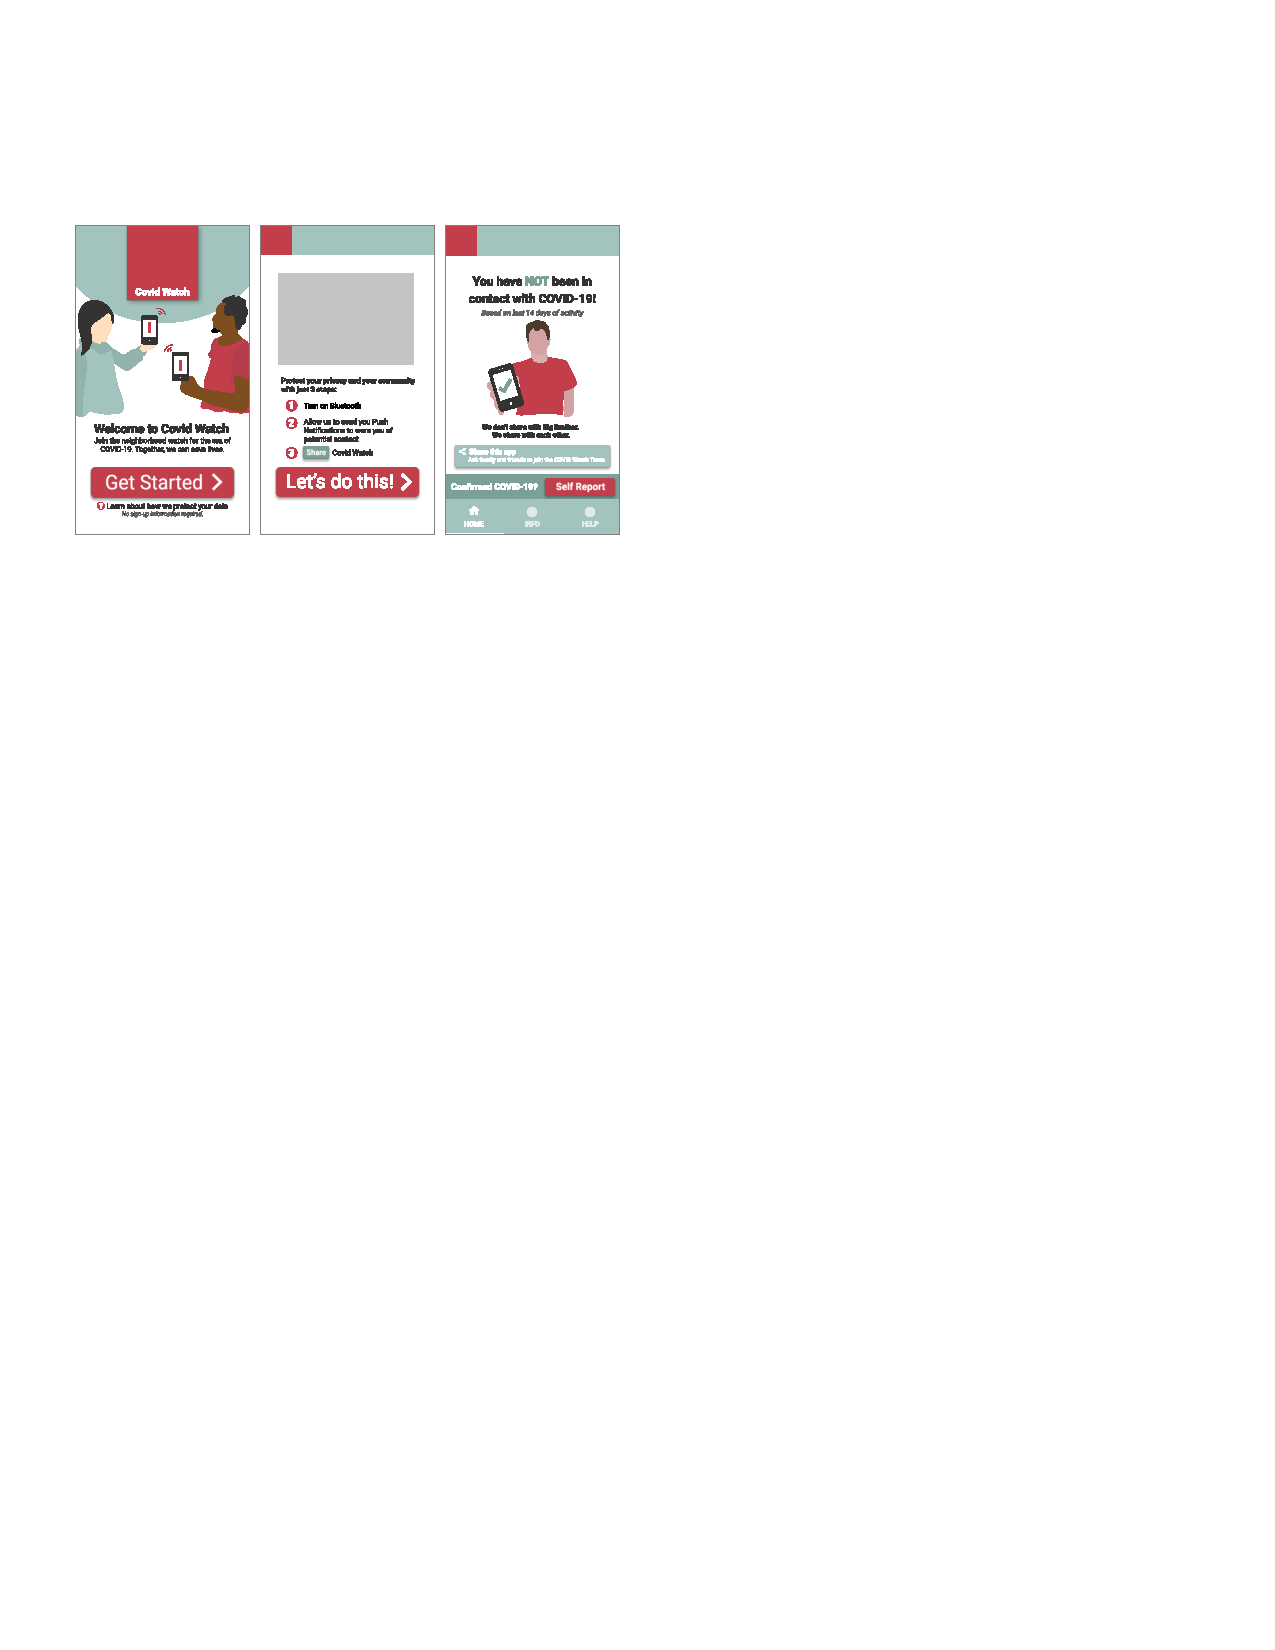
\includegraphics[width=0.5\textwidth]{figs/fig5.pdf} 


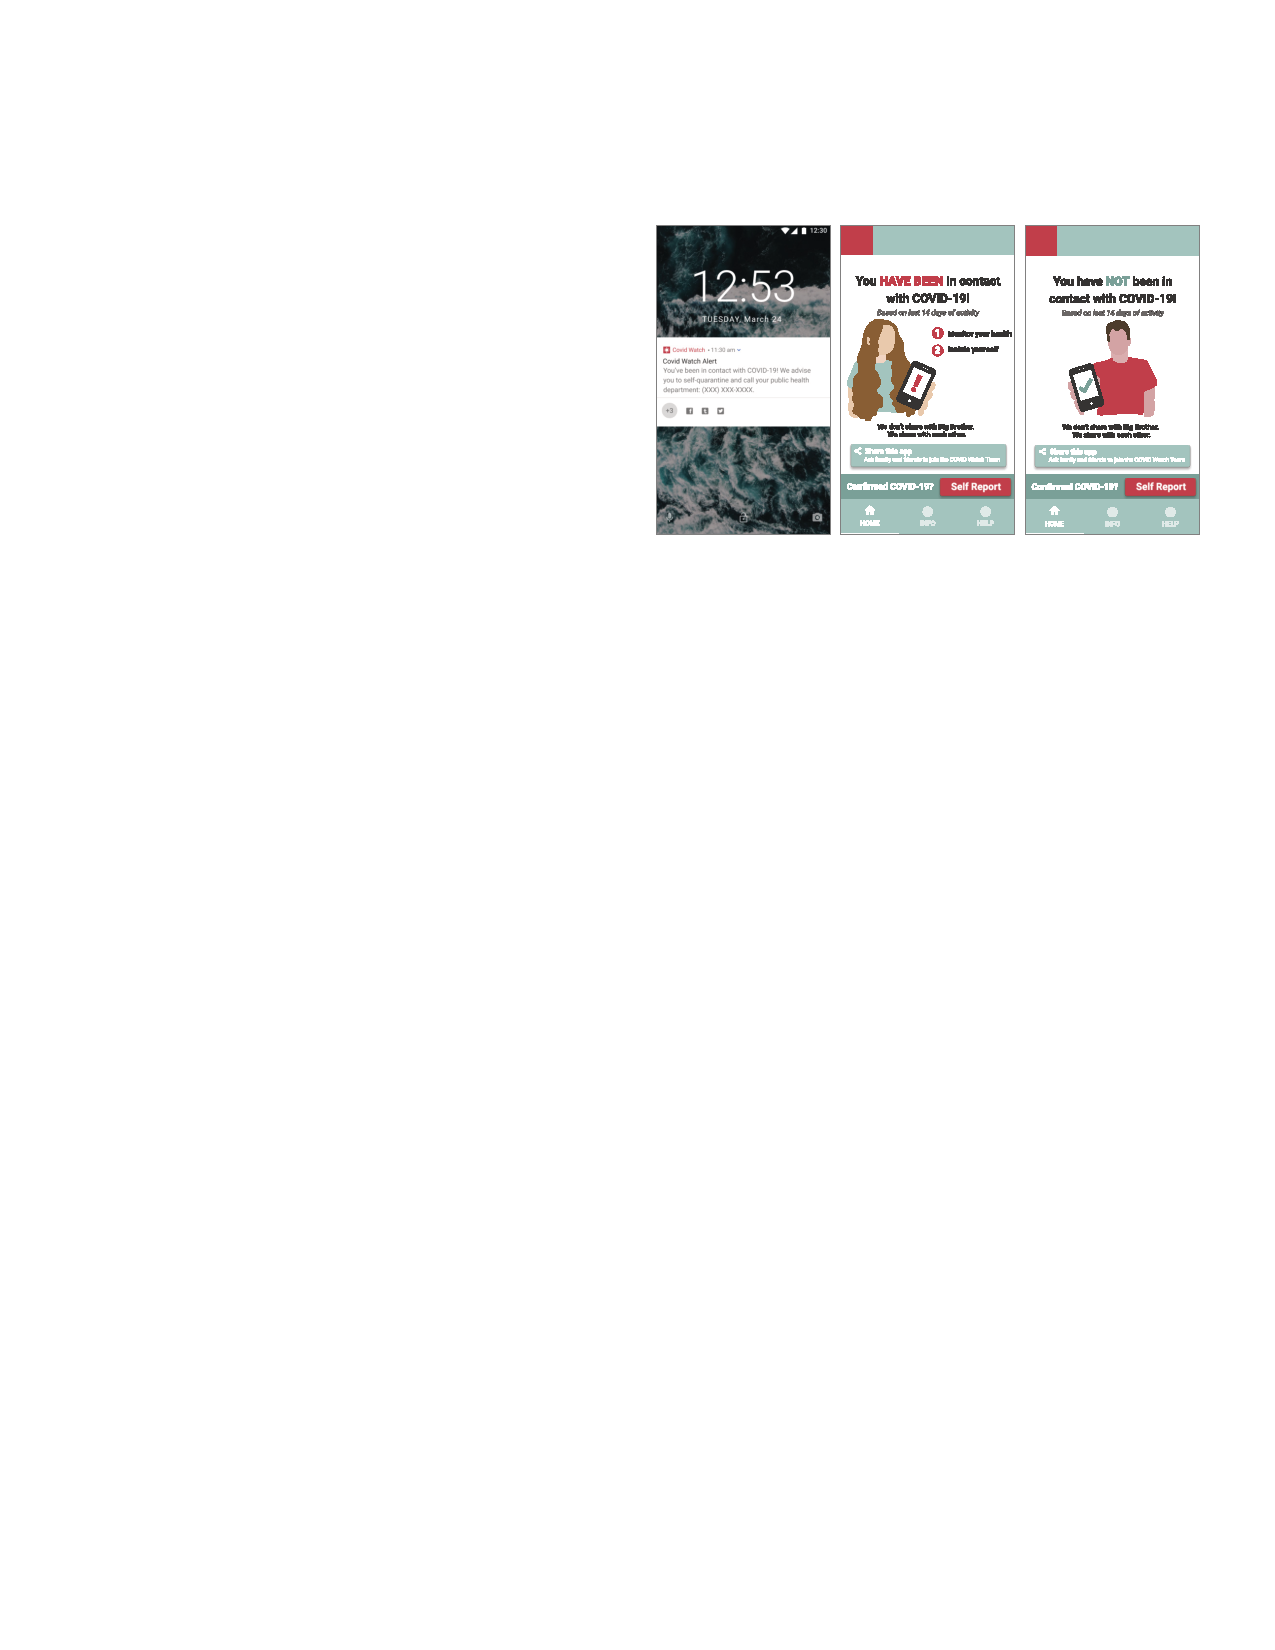
\includegraphics[width=0.5\textwidth]{figs/fig6.pdf}
\caption{\textbf{(top)} User Interface Design: New User OnBoarding Workflow. Downloading and using Covid Watch does NOT require any sign up of email, password, etc. of any kind. The only requirement is to enable Covid Watch to access bluetooth on your smartphone in order to detect other smartphones in close proximity to log a ‘contact event’. If no other smartphones you have been in contact with are associated with a positive case COVID-19, Covid Watch informs you that you have not been in contact with COVID-19.
\textbf{(bottom)} Contact Alert and Reporting. If Covid Watch detects another smartphone within bluetooth proximity that is associated with a positive COVID-19 case, you are alerted that you may have been exposed Covid Watch suggests steps of (1) monitoring your health and (2) isolate yourself. Additionally, you may update your own status as confirmed or not tested, along with the first date of symptoms.}
\end{figure}




\begin{itemize}
  \item CDC general COVID-19 advice, symptoms, and resources
  \item An infection density heat map based on anonymized GPS data
  \item A notification system of potential COVID-19 contact risk via bluetooth proximity networks
  \item Personalized advice: If close contact is detected, a popup instructs the user to call the local public health department, and looks up this number to call for them to inquire about next steps
  \item Future features may include: more personalized advice based on heat map location, a supplies map, self-reporting of symptoms, FAQs, news updates tailored by geographic region, travel counseling, or access to home-based testing
\end{itemize}



\section{Why You Should Care}

\paragraph{Incentives for Health Authorities}
\begin{itemize}
  \item High accuracy, instantaneous contact tracing
  \item Targeted interventions based on calculated risk and current health policy
  \item Easier communication of announcements and information
\end{itemize}


\paragraph{Incentives for Individuals}
\begin{itemize}
  \item Information about how to avoid contracting the disease
  \item Earlier warning to protect friends, family, and close contacts if you do get sick
  \item Friends, family, and close contacts who use the system will likely be warned before they can get you sick
  \item Broad health measures to contain the disease could be relaxed in favor of targeted and private interventions, so regular life will not need to be disrupted as much
\end{itemize}


\subsection{Quantitative Analysis of Impact}


The impact of this technology will depend largely on the state of the world around it. Numerical models~\cite{Ferrettieabb6936} and ongoing campaigns~\cite{normile_2020} suggest that with extensive testing, accurate contact tracing, and isolation of suspected cases, outbreaks can be contained. 

For intermediate testing and contact tracing detection rates, a system like this would likely need to be used in combination with continued social distancing measures and manual contact tracing. However, the measures suggested by Ferguson et al. could potentially be relaxed if supplemented with sufficient targeted interventions.   

Of the three target parameters (tracing accuracy, detection rate, base transmission), the potential influence of the app on tracing accuracy is the simplest to quantify. Any two users of the app who are at the same location at the same time will register a contact event. In theory,  all transmission events except those by fomites would be detected. This includes all types of contact classified as being “high risk” by the ECDC. 

Preventative measures encouraged by the app such as avoiding high-risk areas and increased precautions would reduce overall transmission rate, however it is difficult to quantify this impact. The current design of the app may also increase detection rate by informing users of symptoms to watch for and how to get tested. Ongoing research is being conducted on how to allocate testing resources to maximize the expected value of secondary cases detected. 

To have a significant impact the technology will require a significant adoption rate. To detect contact events using bluetooth both individuals must have the app installed at the time of transmission. Assuming $P$ percent of the population uses the app, $A$  percent of transmission events between app users are detected, and $T$ percent of infected are tested, then $TAP^2$ percent of total transmissions are detected (if app users are homogeneous in the population). 

Figure~\ref{transdect} below examines the percentage of detectable transmission events in countries with different testing rates as a function of app usage. The analysis assumes that these events are uncorrelated, which may significantly under-estimate detected transmissions due to missing chain-reaction testing. Ongoing modeling work is being done to investigate the dynamics of rapid tracing and testing along infection chains.


\begin{figure}[ht]
\centering
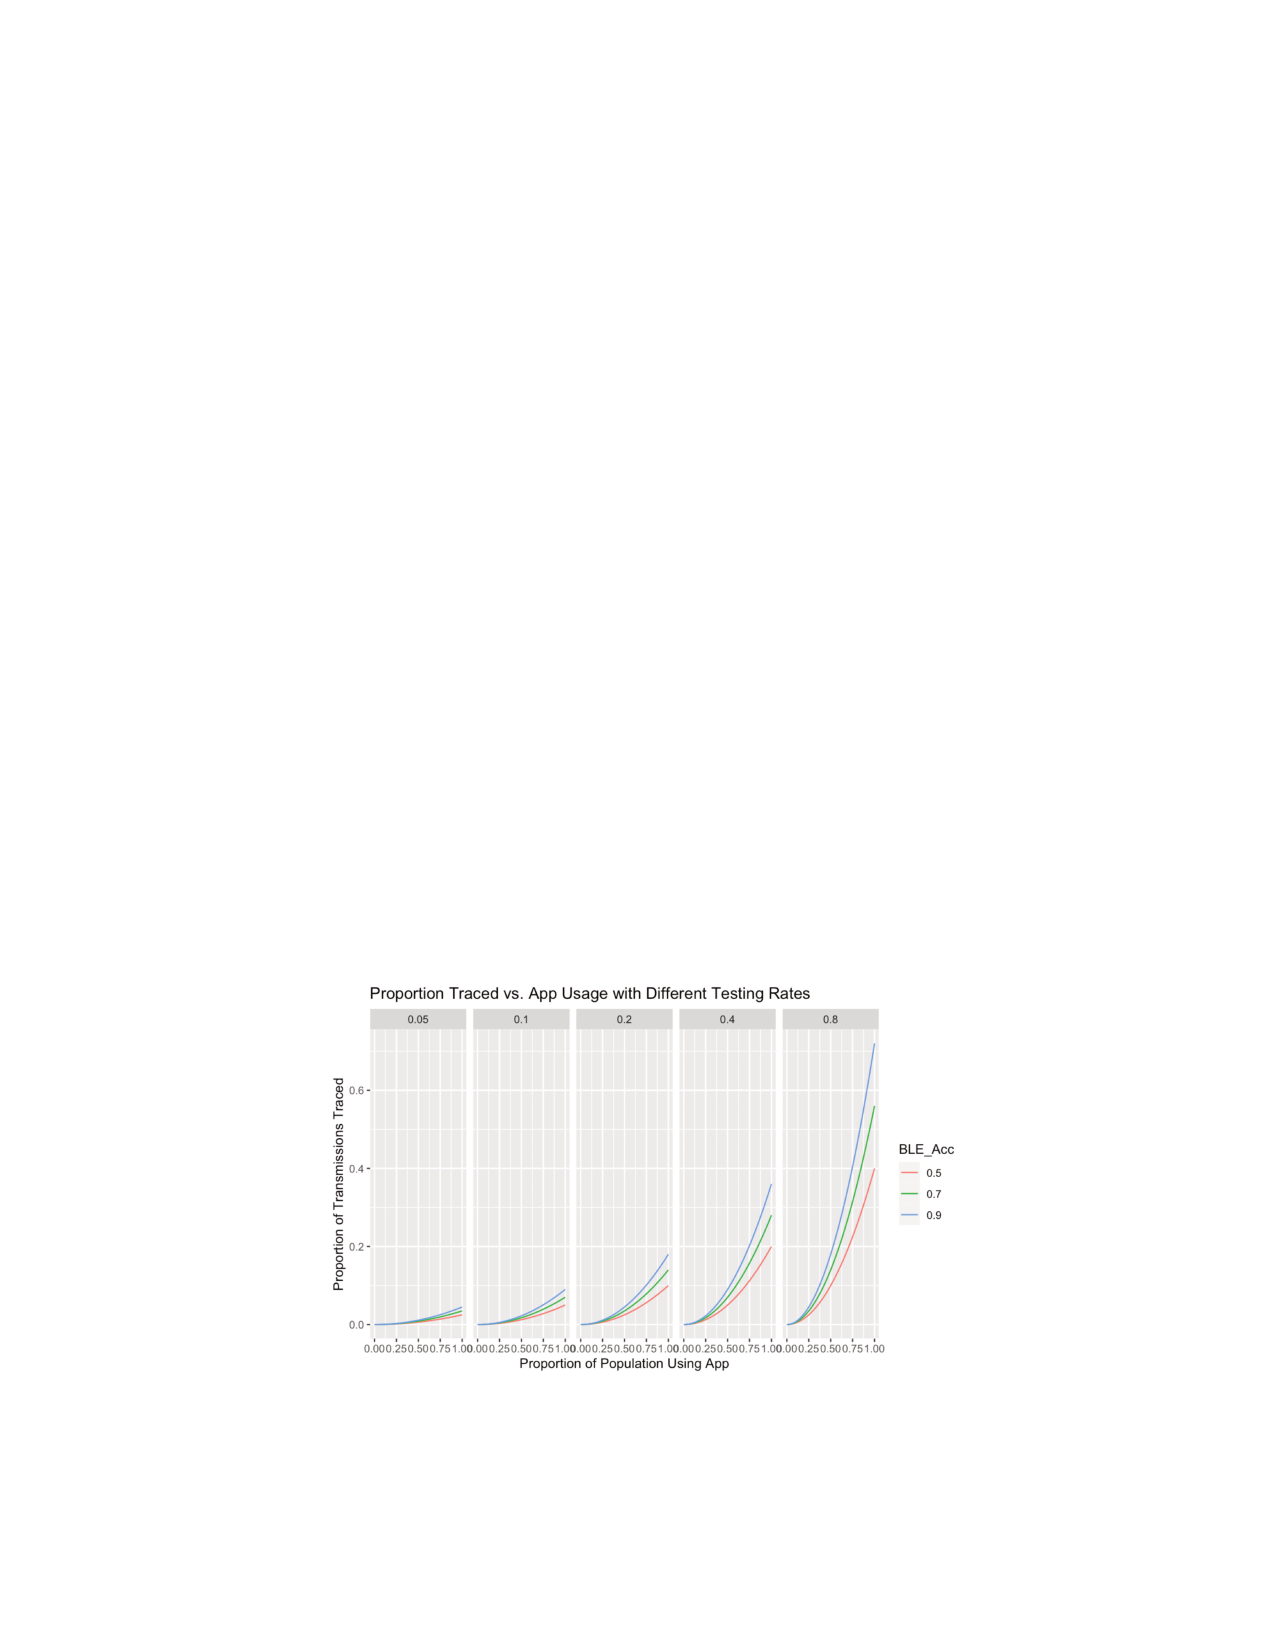
\includegraphics[width=0.8\textwidth]{figs/fig7.pdf} 
\caption{Transmission Detection vs. App Usage curves for testing rates $[0.05, 0.1, 0.2, 0.4, 0.8]$. BLE\_Acc gives the detection rate of transmission events between app users.}
\label{transdect}
\end{figure}


\begin{figure}[ht]
\centering
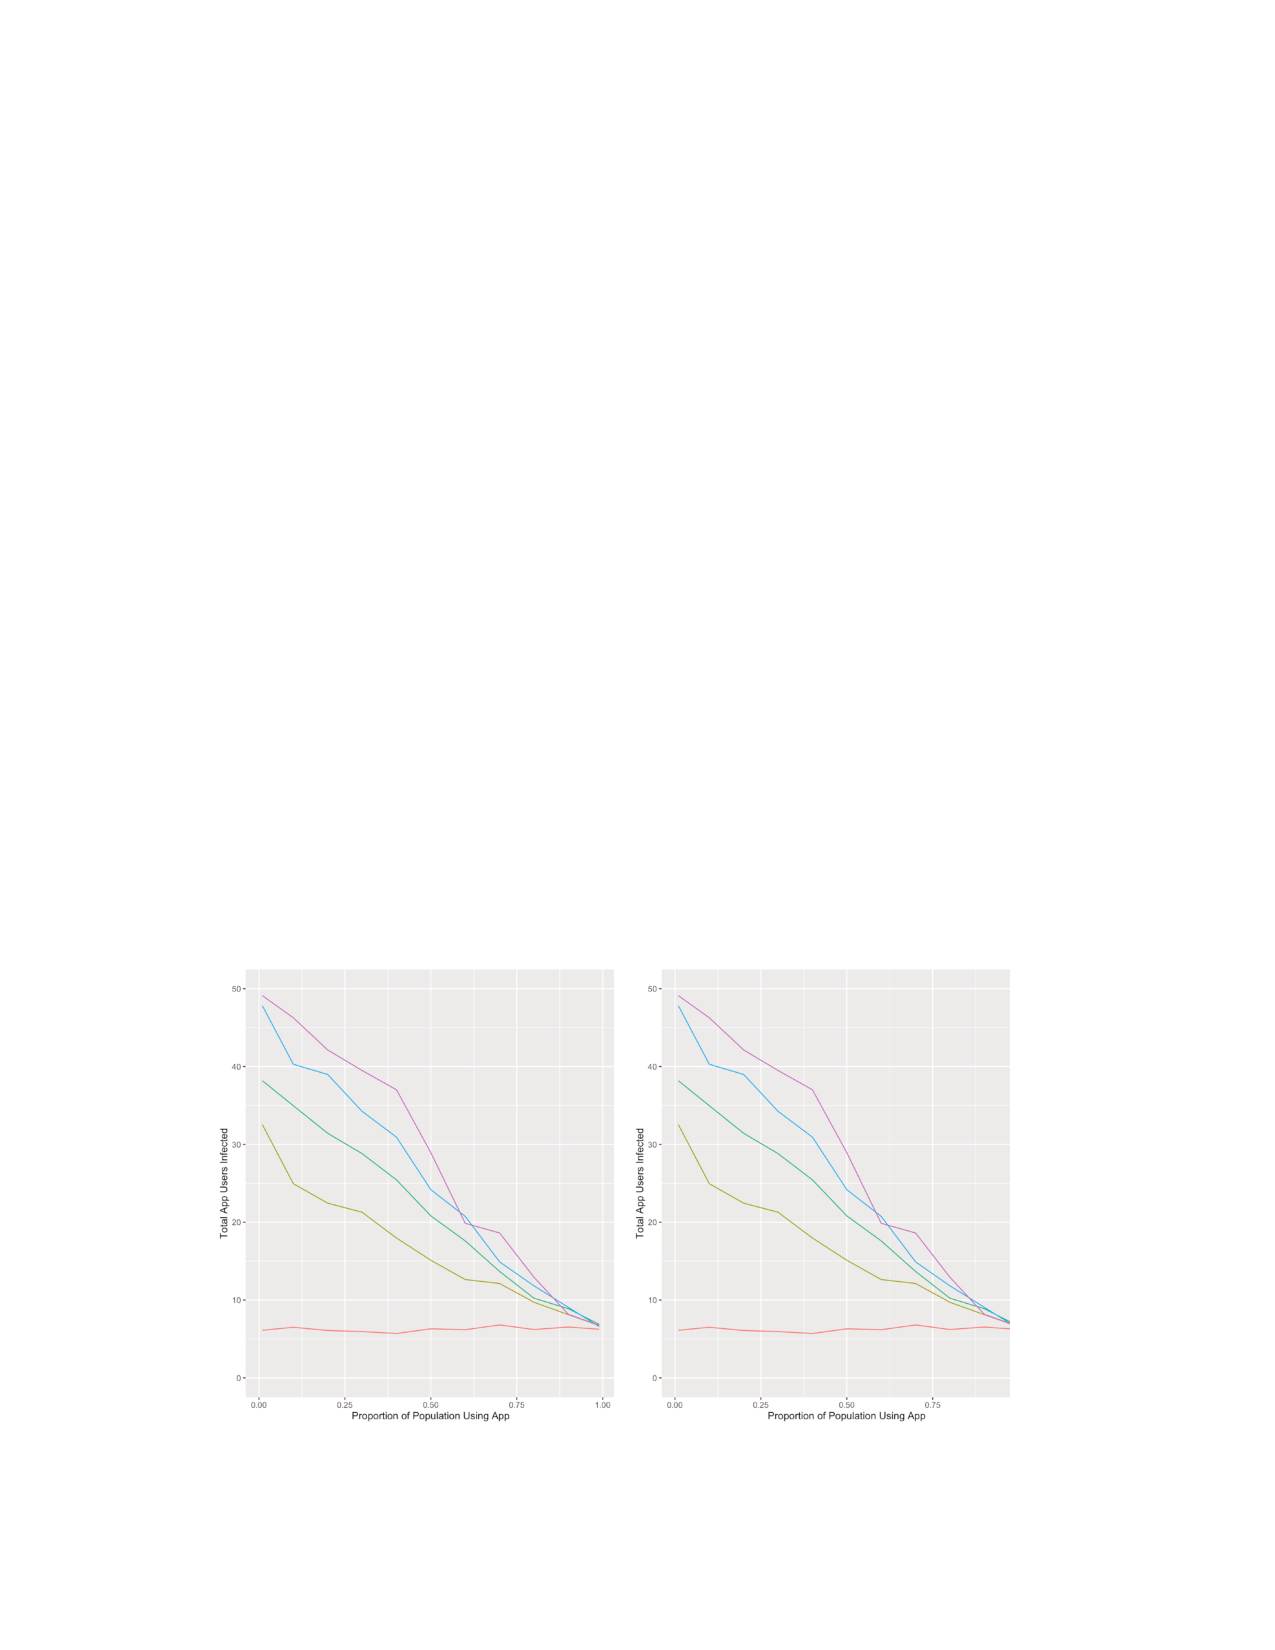
\includegraphics[width=0.8\textwidth]{figs/fig8.pdf} 
\caption{Expected infections for total population (1st) and app population (2nd) adjusted for relative population size.}
\label{expinf}
\end{figure}

In order to investigate disease dynamics with clusters of app users, the model developed by Hellewel et al was modified to account for two sub-populations, one that uses the app and another that doesn’t. The modified implementation is available on Github here and currently assumes 90\% app tracing accuracy and 50\% non-app tracing accuracy (assuming health systems are partially overwhelmed).

Figure~\ref{expinf} was used to estimate the average number of infections caused in 6 weeks due to a single imported case. Results show a significant reduction in risk for clusters of app users that are partially distanced from non app users. This is important because it provides an additional incentive for individuals to use the app even when the overall adoption rate is low. As the proportion of the population using the app increases the risk for the entire population is reduced and most outbreaks are contained. 



What we’ve most wanted to know is the answer to this question: ``Can an effective contact tracing program reduce local transmission so that sustained local spread does not occur?'' The answer looks like yes.
With a comprehensive testing program, high mobile app contact tracing accuracy, and self-isolation of diagnosed individuals, our models predict that each new case could cause on the order of 10 other cases before the outbreak is extinguished. 
Also, even in parameter regimes where automated contact tracing alone is not enough, this technology can be used in combination with existing methodologies to provide greater protection with lower social cost.


\section{Timeline}

We estimate we could complete the remainder of the necessary technical requirements and deploy the first version of the mobile app for pilot within 2 weeks, and possibly sooner, based on the rapid rate of progress that has so far been achieved by the researchers and volunteers who have devoted their time to this technically sophisticated, but potentially high impact intervention. 

The track to development requires (1) more volunteers to help us with skill sets listed on our collaborate page and (2) funding for, at a minimum, cloud services.

The app will be implemented and launched in two parts:

\begin{enumerate}
\item The first version will implement the Bluetooth proximity network and risk heatmap to notify users of potential close contact exposure to SARS-CoV-2.
\item The second version will build upon the initial launch. Users may be able to self-report symptoms to receive personalized advice based on their risk score and advice from the local health department.
\end{enumerate}


We intend to build the tools for all of these systems, but understand that regulatory requirements may vary by region. The app will be designed so that each component can be used separately if necessary.

We also want to emphasize that high user adoption as quickly as possible after release will facilitate the best possible outcomes for intervention. The app may not be able to make use of historical GPS data from individuals, and historical data from bluetooth contact events doesn’t exist. Therefore, a user needs to download the app in order to start the clock and begin benefiting from the system as it anonymously logs bluetooth contact events.


\section{Conclusions}

Mobile technologies can provide instantaneous and high accuracy contact tracing, even between strangers at low social and economic cost. Instead of requiring thousands of healthcare workers to do this manually, the process will be essentially cost-free. Because the system will be so accurate, a majority of people can resume living their lives normally without the need for indefinite social distancing.

We are developing this technology as a high-quality filter to be used for the pandemic optimization problem. Combined with a comprehensive testing program, our filter may be powerful enough to stop further spread of COVID-19. 

\paragraph{Who Can Help} We continue to seek more collaborators, donors, and support from health organizations and testing centers.


% \bibliographystyle{IEEEtran}
% \bibliography{covidwatch}

% Generated by IEEEtran.bst, version: 1.14 (2015/08/26)
\begin{thebibliography}{10}
\providecommand{\url}[1]{#1}
\csname url@samestyle\endcsname
\providecommand{\newblock}{\relax}
\providecommand{\bibinfo}[2]{#2}
\providecommand{\BIBentrySTDinterwordspacing}{\spaceskip=0pt\relax}
\providecommand{\BIBentryALTinterwordstretchfactor}{4}
\providecommand{\BIBentryALTinterwordspacing}{\spaceskip=\fontdimen2\font plus
\BIBentryALTinterwordstretchfactor\fontdimen3\font minus
  \fontdimen4\font\relax}
\providecommand{\BIBforeignlanguage}[2]{{%
\expandafter\ifx\csname l@#1\endcsname\relax
\typeout{** WARNING: IEEEtran.bst: No hyphenation pattern has been}%
\typeout{** loaded for the language `#1'. Using the pattern for}%
\typeout{** the default language instead.}%
\else
\language=\csname l@#1\endcsname
\fi
#2}}
\providecommand{\BIBdecl}{\relax}
\BIBdecl

\bibitem{covidwatch}
\BIBentryALTinterwordspacing
\emph{Covid Watch}, (Accessed 30 May 2020). [Online]. Available:
  \url{https://github.com/covid19risk/}
\BIBentrySTDinterwordspacing

\bibitem{mcneil_2020}
\BIBentryALTinterwordspacing
D.~G. McNeil, ``Inside china’s all-out war on the coronavirus,'' \emph{New
  York Times}, Mar 2020. [Online]. Available:
  \url{https://www.nytimes.com/2020/03/04/health/coronavirus-china-aylward.html}
\BIBentrySTDinterwordspacing

\bibitem{normile_2020}
\BIBentryALTinterwordspacing
D.~Normile, ``Coronavirus cases have dropped sharply in south korea. what’s
  the secret to its success?'' \emph{Science Magazine}, Mar 2020. [Online].
  Available:
  \url{https://www.sciencemag.org/news/2020/03/coronavirus-cases-have-dropped-sharply-south-korea-whats-secret-its-success}
\BIBentrySTDinterwordspacing

\bibitem{ferguson}
\BIBentryALTinterwordspacing
N.~M. Ferguson, D.~Laydon, G.~Nedjati-Gilani, N.~Imai, K.~Ainslie, M.~Baguelin,
  S.~Bhatia, A.~Boonyasiri, Z.~Cucunuba, G.~Cuomo-Dannenburg, A.~Dighe,
  I.~Dorigatti, H.~Fu, K.~Gaythorpe, W.~Green, A.~Hamlet, W.~Hinsley, L.~C.
  Okell, S.~van Elsland, H.~Thompson, R.~Verity, E.~Volz, H.~Wang, Y.~Wang,
  P.~G. Walker, C.~Walters, P.~Winskill, C.~Whittaker, C.~A. Donnelly,
  S.~Riley, and A.~C. Ghani., ``Report 9 - impact of non-pharmaceutical
  interventions (npis) to reduce covid-19 mortality and healthcare demand,''
  Mar 2020. [Online]. Available:
  \url{https://www.imperial.ac.uk/mrc-global-infectious-disease-analysis/covid-19/report-9-impact-of-npis-on-covid-19/}
\BIBentrySTDinterwordspacing

\bibitem{contacttracing_ca}
\BIBentryALTinterwordspacing
\emph{Public health management of cases and contacts associated with
  coronavirus disease 2019 (COVID-19)}, 10 April 2020 (Accessed 30 May 2020).
  [Online]. Available:
  \url{https://www.canada.ca/en/public-health/services/diseases/2019-novel-coronavirus-infection/health-professionals/interim-guidance-cases-contacts.html}
\BIBentrySTDinterwordspacing

\bibitem{lancet}
\BIBentryALTinterwordspacing
J.~Hellewell, S.~Abbott, A.~Gimma, N.~I. Bosse, C.~I. Jarvis, T.~W. Russell,
  J.~D. Munday, A.~J. Kucharski, W.~J. Edmunds, F.~Sun, S.~Flasche, B.~J.
  Quilty, N.~Davies, Y.~Liu, S.~Clifford, P.~Klepac, M.~Jit, C.~Diamond,
  H.~Gibbs, K.~van Zandvoort, S.~Funk, and R.~M. Eggo, ``Feasibility of
  controlling covid-19 outbreaks by isolation of cases and contacts,''
  \emph{The Lancet Global Health}, vol.~8, no.~4, pp. e488--e496, 2020/05/31
  2020. [Online]. Available:
  \url{https://doi.org/10.1016/S2214-109X(20)30074-7}
\BIBentrySTDinterwordspacing

\bibitem{Ferrettieabb6936}
\BIBentryALTinterwordspacing
L.~Ferretti, C.~Wymant, M.~Kendall, L.~Zhao, A.~Nurtay, L.~Abeler-D{\"o}rner,
  M.~Parker, D.~Bonsall, and C.~Fraser, ``Quantifying sars-cov-2 transmission
  suggests epidemic control with digital contact tracing,'' \emph{Science},
  vol. 368, no. 6491, 2020. [Online]. Available:
  \url{https://science.sciencemag.org/content/368/6491/eabb6936}
\BIBentrySTDinterwordspacing

\bibitem{seirs}
\BIBentryALTinterwordspacing
\emph{SEIR and SEIRS models}, Accessed 30 May 2020. [Online]. Available:
  \url{https://www.idmod.org/docs/hiv/model-seir.html}
\BIBentrySTDinterwordspacing

\bibitem{Primault_2019}
\BIBentryALTinterwordspacing
V.~Primault, A.~Boutet, S.~B. Mokhtar, and L.~Brunie, ``The long road to
  computational location privacy: A survey,'' \emph{IEEE Communications Surveys
  and Tutorials}, vol.~21, no.~3, p. 2772–2793, 2019. [Online]. Available:
  \url{http://dx.doi.org/10.1109/COMST.2018.2873950}
\BIBentrySTDinterwordspacing

\bibitem{traject}
\BIBentryALTinterwordspacing
M.~Ghasemzadeh, B.~C. Fung, R.~Chen, and A.~Awasthi, ``Anonymizing trajectory
  data for passenger flow analysis,'' \emph{Transportation Research Part C:
  Emerging Technologies}, vol.~39, pp. 63 -- 79, 2014. [Online]. Available:
  \url{http://www.sciencedirect.com/science/article/pii/S0968090X13002623}
\BIBentrySTDinterwordspacing

\end{thebibliography}



\end{document}